\documentclass [a4paper,12pt,oneside] {report}
\usepackage[colorlinks,linkcolor=black,anchorcolor=black,citecolor=black]{hyperref}
\usepackage{xeCJK}
\usepackage{graphics}

\usepackage{epsfig}

\usepackage{enumerate} %枚举宏包
\usepackage{listings}
\usepackage{geometry}
\usepackage{indentfirst}
\usepackage{xcolor}
\punctstyle{kaiming}
\usepackage{booktabs}
\usepackage{multirow}
\definecolor{mygray}{rgb}{0.3,0.3,0.3}
\definecolor{codegreen}{rgb}{0.8,0.8,0.8}
\vspace{50pt}%调整表格行高
\linespread{1.30}%行间距
\geometry{a4paper,left=2cm,right=2cm,top=1cm,bottom=1.5cm}



%设置字体
%\setmainfont{STKAITI.TTF}
%\setmainfont{Noto Sans CJK JP Thin}
\setmainfont{Ubuntu}
%\setCJKmainfont{SimSun} % 语义和语法同fontspec
%\setCJKsansfont{SimHei}
%\setCJKmonofont{SimSun}


\makeatletter



\lstset{
	numbers=left,
	numberstyle=\tiny,
	basicstyle=\scriptsize,
	backgroundcolor= \color{gray},
	keywordstyle=\color{blue!70},
	breaklines=true,
	breakautoindent=true,
	breakindent=4em,
	commentstyle=\color{codegreen},
	frame=shadowbox,
	escapeinside=``,
	tabsize=4,
	framextopmargin=1pt,framexbottommargin=1pt,abovecaptionskip=-1pt,belowcaptionskip=1pt,
  xleftmargin=3em,xrightmargin=3em,
	language=C
}
\begin{document}


\title{\textbf{UEFI 执行流程}\\ % Title
及 \\BSP Performance Debug} % Subtitle

\author{\textsc{haobo.gao} % Author
\\{\textbf{Foxconn ZZDC}}} % Institution

\date{\today} % Date
\maketitle


\pagenumbering{roman}
\tableofcontents
\newpage
\pagenumbering{arabic}
\chapter{Bsp Performance Debug}


前段时间,我尝试帮助分析了PL2P-2393 关于
\begin{lstlisting}
("Power On to home screen (for 2nd boot or later)"is worse than PL2O.(PL2P: 37.52sec, PL2O: 31.26sec))
\end{lstlisting}
Performance方面的一个 issue.接下来
和大家分享下过程中遇到的问题和得到的经验。


\section{思路}




\subsection{控制硬件及其参数配置不变}
首先用最好使用同一台手机,进行问题复现。
这样能确定硬件的一致。


在硬件一致的前提下,我们首先要确定软件
方面对于硬件方面的配置是否有差异。根据
我的认知,以下三方面的硬件差异会对Perf
ormance造成影响:

\begin{itemize}

\item CPU的频率

\item memory的大小及频率

\item flash 的 Throughput(吞吐量)

\end{itemize}


由于是同一台手机,所以硬件因素是可以保证的。关于参数的配置
通过uefi log 的打印 我们可以看到log 中存在:
\begin{lstlisting}
S - Core 0 Frequency, 3952 MHz
S - Flash Throughput, 80000 KB/s  (4694664 Bytes,  58271 us)
DDR Frequency, 1296 MHz
Core 0 Freq: 1670400 MHz
\end{lstlisting}

要确认以上参数的一致,不过发现Flash Throughput 会有小范围浮动,
不足以造成很大的差异。

\subsection{kernel 配置}
 
在确定软件对于硬件的配置参数都一样的情况下,我们也要确认一下使用的kernel 编译配置。kernel 有两种编译配置,
一种用在开发阶段是sdm660\_defconfig。这种配置编译出来的kernel 中有一些debug 信息,高通文档描述说 是 
has bad performance。还有一种用于产品阶段的配置,sdm660-perf\_defconfig  这个配置摘掉了debug info
为  good performance。

编译一个userdebug版本 bad performance:
\begin{lstlisting}
TARGET_BUILD_VARIANT=userdebug
\end{lstlisting}

编译一个user版本 good performance:
\begin{lstlisting}
TARGET_BUILD_VARIANT=user
\end{lstlisting}

\subsection{版本升级因素}
考虑可能是版本升级代码变动造成
的影响。我们需要抓取log 锁定问题的范围。




 

\section{本文必备的uefi基础}

为了能看懂log ,需要对uefi 启动流程做一个大致的介绍,由于我还没有完全
把我看到的文档解释和uefi的源码对应起来,很多地方还存在疑惑,所以并不能
详细介绍uefi的启动流程。但是现阶段可以确定的部分足以用来处理这个问题。


\subsection{uefi 组件}


\subsubsection{xbl 的源代码目录}
位于 BOOT.XF.1.4/boot\_images/目录下的 代码编译可以生成xbl.elf 和 pmic.elf 等 \ref{xbldir}:
\begin{figure}
\begin{center}
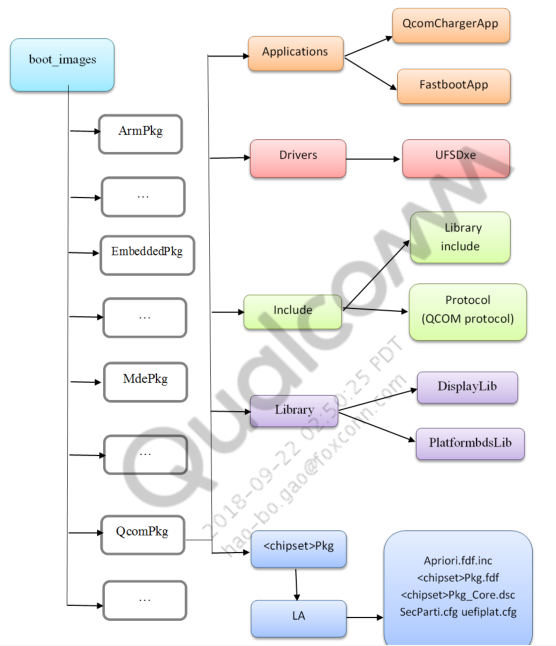
\includegraphics[width=10cm]{img/xbldir}
\caption{xbl 目录}
\label{xbldir}
\end{center}
\vspace{-0.5em}
\end{figure}


\subsubsection{abl 的源代码目录}
位于LINUX/android/bootable/bootloader/edk2/ 目录下的 代码编译成为abl.elf \ref{abldir}:
\begin{figure}
\begin{center}
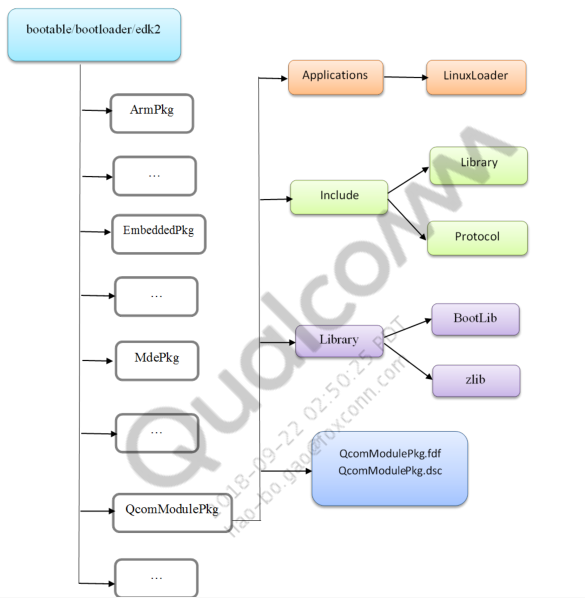
\includegraphics[width=10cm]{img/abldir}
\caption{abl 目录}
\label{abldir}
\end{center}
\vspace{-0.5em}
\end{figure}


\subsubsection{效果图}
以下是 效果图\ref{howxblmade}。
\begin{figure*}[htbp]
\begin{center}
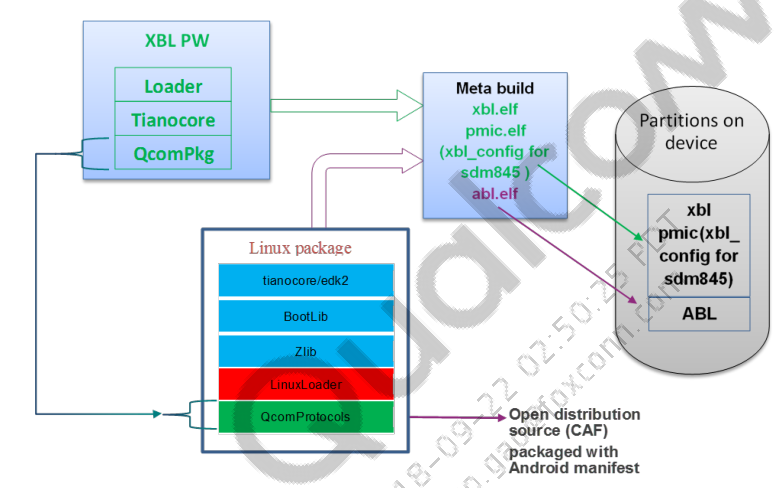
\includegraphics[width=10cm]{img/uefimeta}
\caption{uefi build chat}
\label{howxblmade}
\end{center}
\vspace{-0.5em}
\end{figure*}


\subsection{xbl region}

\subsubsection{ xbl 的编译过程 }
下图\ref{madexbl}简单展示了XBL是如何被编译成为elf 文件的。

\begin{figure*}[htbp]
\begin{center}
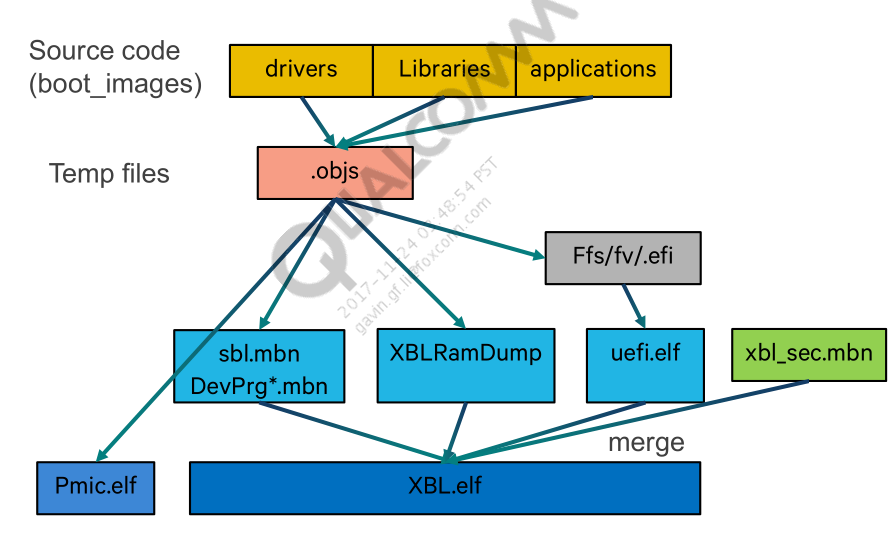
\includegraphics[width=10cm]{img/madexbl}
\caption{xbl made for}
\label{madexbl}
\end{center}
\vspace{-0.5em}
\end{figure*}


\subsubsection{xbl region}
xbl.elf 中有4个域\ref{xblreg}。

\begin{figure*}[htbp]
\begin{center}
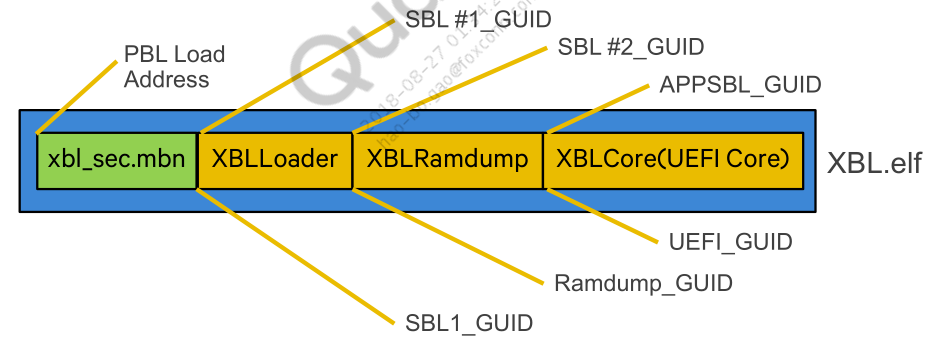
\includegraphics[width=10cm]{img/xbl_reg}
\caption{xbl region}
\label{xblreg}
\end{center}
\vspace{-0.5em}
\end{figure*}









\subsection{uefi 执行流程}


图\ref{xblstage}表示uefi 执行的阶段。sec 相关的 region 最先被执行。
接下来 会去加载 DXE ,也就是驱动。到BDS (boot device select)时,会
检测hot key,并执行与hot key 对应的动作。 本次我们讨论的是加载abl。
接着,由Android源码目录下的 edk2 编译生成的abl.elf 中的linux\_loader
完成HLOS 的加载和执行。uefi boot serveice 结束。

\begin{figure*}[htbp]
\begin{center}
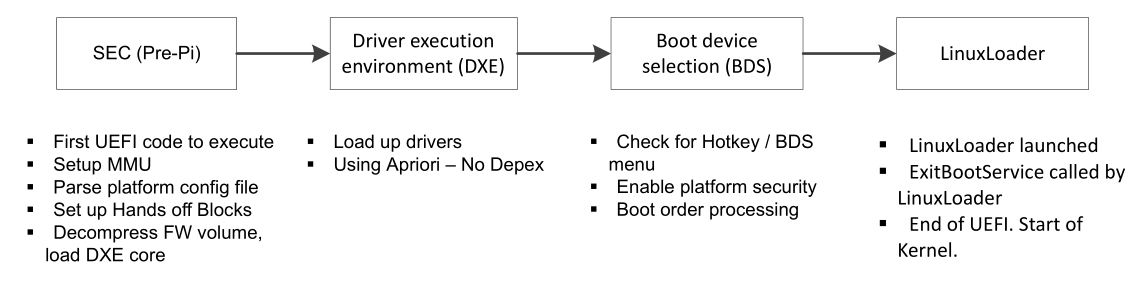
\includegraphics[width=15cm]{img/uefistage}
\caption{uefi 阶段}
\label{xblstage}
\end{center}
\vspace{-0.5em}
\end{figure*}




\section{代码位置以及log片段介绍}

这里介绍uefi一些阶段对应的 log 以及其对应的代码。

\subsection{UEFI Start 之前的log}

如果你使用串口抓取log ,是不会看到有\ref{loaderinfo},所
列举的log. 这是因为在xbl loader 编译的时候没有打开FEATURE\_BOOT\_LOGGER\_UART
编译选项,所以对于早期的串口打印函数 比如boot\_log\_message\_raw. 在没有打开
这个选项的时候,用于串口打印的 inline 函数被声明为一个空的函数体。所以同样的log 
仅仅通过boot\_log\_message\_ram 记录在log buffer 中 随后某个时间 被插入到 blog 的
开始部分。








如果十分想要看这部分的串口log,又没有更好的方法,请尝试
在
\begin{lstlisting}
boot_images/QcomPkg/Sdm660Pkg/Library/XBLLoaderLib/XBLLoaderDevProgLib.inf
\end{lstlisting}
 文件中,找到如下文本片段:
\begin{lstlisting}
[BuildOptions.AARCH64]
GCC:*_*_*_CC_FLAGS = -Werror -DBOOT_LOADER -DBOOT_WATCHDOG_DISABLED -DBOOT_PBL_H=\"pbl_sbl_shared.h\"  -DBUILD_BOOT_CHAIN -DRAM_PARTITION_TABLE_H=\"ram_partition.h\" -DBOOT_INTERNAL_HEAP_SIZE=0x01800 -DBOOT_EXTERNAL_HEAP_SIZE=0x10000 -DFEATURE_BOOT_SDCC_BOOT -DFEATURE_BOOT_LOAD_ELF -DFEATURE_BOOT_SKIP_ELF_HASH_VERIFICATION -DFEATURE_BOOT_VERSION_ROLL_BACK -DUSE_GNU_LD -DUSE_LOADER_UTILS   -DFEATURE_BOOT_LOGGER_RAM -DFEATURE_BOOT_LOGGER_TIMER -DFEATURE_BOOT_LOGGER_JTAG -DFEATURE_BOOT_LOGGER_UART -DFEATURE_BOOT_EXTERN_SECIMG_AUTH_COMPLETED -DFEATURE_DEVICEPROGRAMMER_IMAGE
MSFT:*_*_*_CC_FLAGS = -DBOOT_LOADER -DBOOT_WATCHDOG_DISABLED -DBOOT_PBL_H=\"pbl_sbl_shared.h\"  -DBUILD_BOOT_CHAIN -DRAM_PARTITION_TABLE_H=\"ram_partition.h\" -DBOOT_INTERNAL_HEAP_SIZE=0x01800 -DBOOT_EXTERNAL_HEAP_SIZE=0x10000 -DFEATURE_BOOT_SDCC_BOOT -DFEATURE_BOOT_LOAD_ELF -DFEATURE_BOOT_SKIP_ELF_HASH_VERIFICATION -DFEATURE_BOOT_VERSION_ROLL_BACK -DUSE_GNU_LD -DUSE_LOADER_UTILS   -DFEATURE_BOOT_LOGGER_RAM -DFEATURE_BOOT_LOGGER_TIMER -DFEATURE_BOOT_LOGGER_JTAG -DFEATURE_BOOT_LOGGER_UART -DFEATURE_BOOT_EXTERN_SECIMG_AUTH_COMPLETED -DFEATURE_DEVICEPROGRAMMER_IMAGE
\end{lstlisting}
并在 对应的位置 添加 -DFEATURE\_BOOT\_LOGGER\_UART 编译选项。
\begin{lstlisting}
#ifdef FEATURE_BOOT_LOGGER_UART
void boot_log_message_uart(char *, uint32, char, char *);
#else
static inline void boot_log_message_uart(char * m, uint32 t, char l, char * c)
{
}
#endif

void boot_log_message_raw(char * message,uint32 timestamp,char log_type,char * optional_data)
{
  /*Logs message with time stamp in ram, must be initialized first.*/
  boot_log_message_ram(message,timestamp,log_type,optional_data);
  /* Transmit the message with time stamp */
  boot_log_message_uart(message,timestamp,log_type,optional_data);
}
\end{lstlisting}


\subsubsection{PBL LOG}
关于这部分log 中出现的: 
\begin{lstlisting}
PBL, Start
PBL, End
\end{lstlisting}

容易让人怀疑 PBL 在执行的时候是否打印出了如下的log。并且在代码中搜索
相关字符串,居然能搜索到。 根据 高通文档描述 我们这里应该是没有PBL 部分
的源码的,PBL 是固化到Rom中的一小段程序。

经过追查发现,如下代码解释了这个问题:
\begin{lstlisting}
/*@brief
*   This funcion will parse the PBL timestamp milestones passed to SBL
*   and insert them into the boot log.  Currently PBL's unit of measure is
*   clock ticks.  PBL does not pass the clock frequency yet so it is hard
*   wired to 19.2 Mhz.  Also PBL does not pass the names of each field so for
*   now reference a structure of our own to get the names which will have
*   logic ready for the day PBL starts passing them.
*/
void boot_pbl_log_milestones(boot_pbl_shared_data_type * pbl_shared_data)
{
	...
  for (count = 0;count < (sizeof(pbl_shared_data->timestamps) / sizeof(uint32));count++, pbl_timestamp++)
  {
    pbl_us_value = ( ( (uint64)(*pbl_timestamp) ) * PS_PER_PBL_TIMESTAMP_TICK ) / 1000000;
    /*Logs message and time. */
    boot_log_message_raw(boot_log_pbl_milestone_names[count],(uint32)pbl_us_value,LOG_MSG_TYPE_BOOT,NULL);
  }
	...
}
\end{lstlisting}
这部分代码打印了那段log ,注释上大意是, 这个函数会去把PBL 传递过来(SBL)的时间
戳数据加到bootlog中。 PBL 时期的时钟是连接到19.2MHZ,并且PBL 并没有把每个时间戳对应
的名字传递过来,所以在SBL 中需要自己定义一组这样的名字。



\subsubsection{高通启动流程}

参见\ref{sdm660boot}.boot详细流程感兴趣的可以去看高通
的相关文档\footnote{80\_P8754\_2\_D\_SDM660\_SDM630\_BOOT\_AND\_COREBSP\_ARCHIT.pdf}
我在这里仅仅简要介绍。
\begin{figure*}[htbp]
\begin{center}
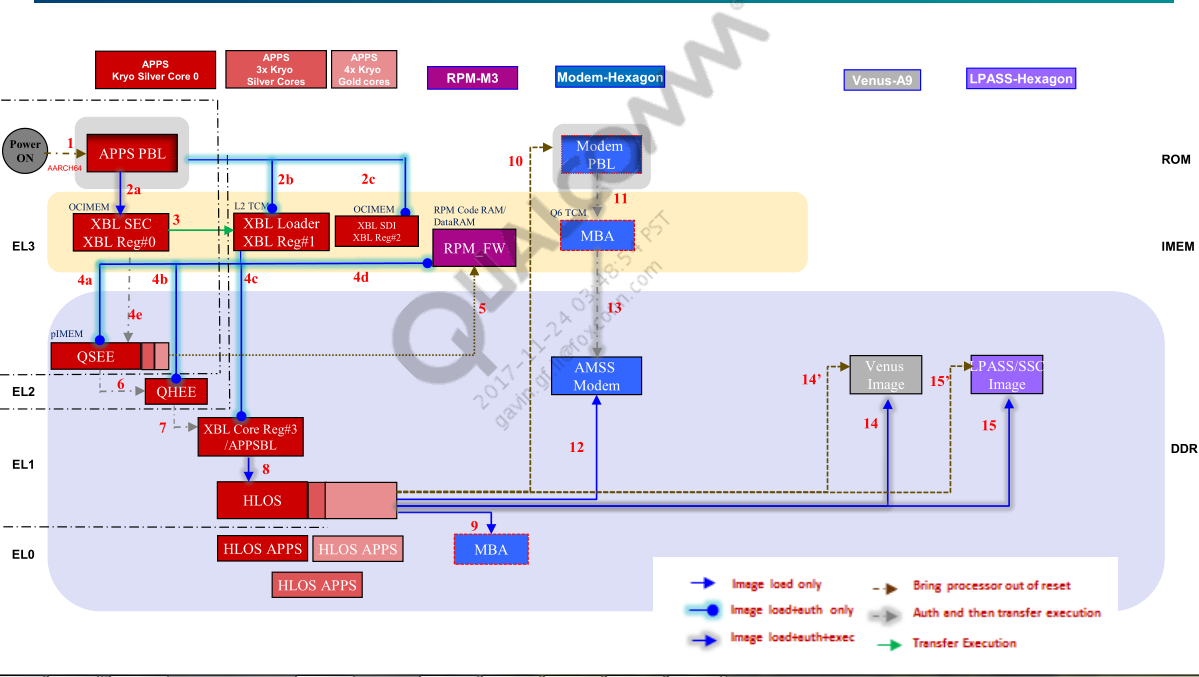
\includegraphics[width=16cm]{img/bootarch}
\caption{SDM660 boot flow}
\label{sdm660boot}
\end{center}
\vspace{-0.5em}
\end{figure*}


\subsection{xbl loader}

从有log 打印开始 已经在xbl loader 中了。

boot\_images/QcomPkg/Sdm660Pkg/Library/XBLLoaderLib/sbl1\_mc.c
\begin{lstlisting}
sbl1_main_ctl
\end{lstlisting}

log\ref{loaderinfo} 是由 sbl1\_main\_ctl 的执行产生的 ,sbl1\_main\_ctl 是xbl\_loader 的主体。
主要完成了ram 的配置和初始化,初始化了堆栈,内存映射,qsee 接口。设置hash 运算
检测是否使能secboot。然后通过
boot\_config\_process\_bl\ref{boot_config_process_bl}
跳去执行sbl1\_config\_table 中定义的动作, 见代码\ref{sbl1_config_table}。
在boot\_config\_process\_bl 中在for 循环中调用了 boot\_config\_process\_entry, 处理每一个 在sbl1\_config\_table上的表项。
具体做了:
\begin{itemize}
 \item 执行每一个表项中的pre\_procs。这个函数会在加载镜像前执行。
 \item 检查 boot\_load\_cancel 是否被注册(指向一个函数),有时候注册表中可能会注册这样一个类型的
 函数检查镜像的加载是否该被取消。
 \item 执行Load/Authenticate,根据image type 我们加载认证镜像。
 \item Execute,如果configuration table 中的excute 是 TURE ,将在load 和Authenticate之后
立刻执行exec\_func。这个动作是和下文提到的jump 是互斥的。
 \item Execute post\_procs ,在被加载认证执行之后,执行 post\_procs.
 \item 如果 configuration table 中的 jump 是 TURE ,会在 post\_procs 之后执行jump\_func.
 这个动作是和上文提到的execute 相互斥。	
 
\end{itemize}

以上 这个步骤对应了图\ref{sdm660boot}中的 :
\begin{itemize}
\item 4a. Loads and authenticates the QSEE image from the boot device to ​pIMEM​.
\item 4b. Loads and authenticates the QHEE image from the boot device to DDR.
\item 4c. Loads and authenticates the XBL Core (region \#3) and ABL image from the boot device to
DDR.
\item 4d. Loads and authenticates the RPM firmware image from the boot device to RPM code
RAM.
\item 4e. XBL SEC transfers execution to QSEE.
\end{itemize}


之后控制权qsee qsee 再去执行Qhee 然后控制权交给XBL core。
这部分没有log 也没有在代码中找到相关代码。


\subsection{XBL core}

xbl core 接管控制权后,程序的执行流已经来到了,boot\_images/QcomPkg/XBLCore/Sec.c
中的Main函数。紧跟这的一些打印:
\begin{lstlisting}
UEFI Start     [  757] SEC
\end{lstlisting}
其中的DisplayEarlyInfo
\begin{lstlisting}
UEFI Ver    : 4.2.180915.BOOT.XF.1.4-00258-S660LZB-1
Build Info  : 64b Sep 15 2018 16:39:17
Boot Device : eMMC
\end{lstlisting}

在main结尾 会有这样一个调用
\begin{lstlisting}
LoadDxeCoreFromFv (NULL, 0);
\end{lstlisting}
这个函数会去加载 DxeCore.efi ,然后去执行它。




现在 进入了DXE阶段
DXE阶段的入口为DxeMain,其中起了一些服务配置了一些表。
然后通过:
\begin{lstlisting}
Status = FwVolBlockDriverInit (gDxeCoreImageHandle, gDxeCoreST);
\end{lstlisting}
加载并执行了其他的一些.efi文件(DRIVER),这是dxe 的重要部分(加载驱动并执行),
其中包含:
\begin{lstlisting}
 - 0x09B8D3000 [  916] FIHDxe.efi
\end{lstlisting}

在 DxeMain 的最后 有:
\begin{lstlisting}
gBds->Entry (gBds);
\end{lstlisting}

通过前面加载的QcomBds.efi,已经被配置为如下
\footnote{代码在BOOT.XF.1.4/boot\_images/QcomPkg/Drivers/BdsDxe/BdsEntry.c}:
\begin{lstlisting}
 EFI_BDS_ARCH_PROTOCOL  gBds = {
  BdsEntry
};
\end{lstlisting}
  
  


 
  
\subsection{BDS}  
现在 程序来到了BDS(boot device select)阶段。 
在 BdsEntry\footnote{boot\_images/QcomPkg/Drivers/QcomBds}\ref{BdsEntry} 中

在 BDS 的最后通过LaunchDefaultBDSApps 加载执行:
\begin{itemize}
\item QcomChargerApp.efi

\item FIHHWIDApp.efi

\item LinuxLoader.efi 

\end{itemize}



\subsection{ABL/linuxloader }
最后来到了abl 中的 LinuxLoaderEntry
\begin{lstlisting}
ENTRY_POINT                    = LinuxLoaderEntry
LinuxLoaderEntry
\end{lstlisting}

这里面有fih 添加的很多标有fih\_的函数。
判断BootReason 属于
\begin{lstlisting} 
  NORMAL_MODE = 0x0,
  RECOVERY_MODE = 0x1,
  FASTBOOT_MODE = 0x2,
  ALARM_BOOT = 0x3,
  DM_VERITY_LOGGING = 0x4,
  DM_VERITY_ENFORCING = 0x5,
  DM_VERITY_KEYSCLEAR = 0x6,
  FACTORY_MODE        = 0x7,
  OEM_RESET_MIN = 0x20,
  OEM_RESET_MAX = 0x3f,
  EMERGENCY_DLOAD = 0xFF,
\end{lstlisting}
中哪一类 。
  
最后:
\begin{lstlisting}  
BootLinux (&Info);
\end{lstlisting}

  
\subsection{ dmesg log 中挂接根文件系统开始init 进程的标志 }

在dmesg中 kernel挂接到根文件系统,开始init 进程的标志是:
\begin{lstlisting}
[    1.345851] VFS: Mounted root (ext4 filesystem) readonly on device 252:0.
[    1.347865] Freeing unused kernel memory: 8192K
[    1.396266] init: init first stage started!
\end{lstlisting}





\section{几种log的分析}


\subsection{dmesg}

抓取方法:
\begin{lstlisting}
adb shell dmesg > dmesg.txt
\end{lstlisting}


\subsubsection{KPI(Key Performance Indicator)的计算}

我们可以通过dmesg中的KPI 信息计算出boot loader 的时间,
dmesg 中会有一些类似于 这样的log:
\begin{lstlisting}
[    0.231817] KPI: Bootloader start count = 63197 			\\A begin at edk
[    0.231822] KPI: Bootloader end count = 313686  			\\B end of edk
[    0.231828] KPI: Bootloader display count = 3689772022
[    0.231833] KPI: Bootloader load kernel count = 7456
[    0.231840] KPI: Kernel MPM timestamp = 326766			\\C end of boot loader
[    0.231845] KPI: Kernel MPM Clock frequency = 32768		\\D clock
\end{lstlisting}

根据高通的文档\footnote{kba-160919232945\_3\_how\_to\_debug\_boot\_time\_performance\_issue}的关于KPI计算方面的
描述,我们可以计算出如下信息:

\begin{itemize}

\item NHLOS time : A/D = 1.93S

\item abl time: (B-A)/D = 7.64S	可以从下文的 9558-710 = 7641 得到验证。

\item Boot loader: C/D-kmsg(C)\footnote{标记C的打印时刻,即0.231840} = 9.97 - 0.23 = 9.74s

\end{itemize}








\subsection{Other Kernel part}

必要的时候我们也想知道内核每个模块的加载时间。从而判断
是不是模块加载浪费了时间。


为了达成这个目的 我们需要在 
\begin{lstlisting}
/LINUX/android/kernel/init/main.c

int __init_or_module do_one_initcall(initcall_t fn)
\end{lstlisting}
中的:
\begin{lstlisting}
	if (initcall_debug)
		ret = do_one_initcall_debug(fn);
\end{lstlisting}

把initcall\_debug  替换为 1.

即:
\begin{lstlisting}
	if (1)
		ret = do_one_initcall_debug(fn);
\end{lstlisting}

initcall\_debug 本身是一个bool 类型的变量,在这里强制使
执行流来到do\_one\_initcall\_debug 这样就可以在dmesg 中看到一些
各个模块加载的时间信息了:
\begin{lstlisting}
initcall msm_serial_hsl_init+0x0/0xac returned 0 after 262555 usecs
initcall fts_driver_init+0x0/0x20 returned 0 after 171317 usecs
initcall ufs_qcom_phy_qmp_20nm_driver_init+0x0/0x20 returned 0 after 2572 usecs
initcall ufs_qcom_phy_qmp_14nm_driver_init+0x0/0x24 returned 0 after 1727 usecs
initcall ufs_qcom_phy_qmp_v3_driver_init+0x0/0x24 returned 0 after 1010 usecs
initcall ufs_qcom_phy_qrbtc_v2_driver_init+0x0/0x24 returned 0 after 838 usecs
\end{lstlisting}





\subsection{uefi log}
抓取方法:
\begin{lstlisting}
adb shell cat /proc/blog>E:\uefi.txt
\end{lstlisting}
亦可以使用串口线抓取。

一般情况下 我们直接取到的 uefi 的 log 中已经包含了一些时间戳信息。
\begin{lstlisting}
UEFI Start     [  710] SEC
Render Splash  [ 1729]
Platform Init  [ 1889] BDS
UEFI Total : 1207 ms
POST Time      [ 1917] OS Loader
Loading Image Start : 2996 ms
Loading Image Done : 2996 ms
Total Image Read size : 512 Bytes
Loading Image Start : 2996 ms
Loading Image Done : 3224 ms
Decompressing kernel image start: 8264 ms
Decompressing kernel image done: 8612 ms
Shutting Down UEFI Boot Services: 8762 ms
Exit BS        [ 9558] UEFI End
\end{lstlisting}





\subsubsection{Build A Debug version}


通过修改boot\_images/scripts/build\_boot\_images.sh中的编译条件,可以
得到打印信息更为丰富的uefi log.

\begin{lstlisting}
  -r --release
      Provide a release mode, one of "DEBUG" or "RELEASE". Default is to build both.
\end{lstlisting}



在boot\_images/scripts/build\_boot\_images.sh 中找到如下文本片段,把其中的 RELEASE 改变为 DEBUG.
\begin{lstlisting}
# build xbl -----------------------------------------------

cd $root

cd ../boot_images/QcomPkg/Sdm660Pkg
python ../buildit.py --variant LA -r DEBUG -t Sdm660Pkg,QcomToolsPkg --build_flags=cleanall 2>&1 | tee -a $root/out/$PROJ_NAME-0-$MAJOR_VER$MINOR_VER-build_xbl1.log
python ../buildit.py --variant LA -r DEBUG -t Sdm660Pkg,QcomToolsPkg 2>&1 | tee -a $root/out/$PROJ_NAME-0-$MAJOR_VER$MINOR_VER-build_xbl1.log

# copy image ----------------------------------------------

src=$root"/QcomPkg/Sdm660Pkg/Bin/660/LA/DEBUG"
\end{lstlisting}




更改之后,编译出的DEBUG 版本,log会多出来一些
信息,比如:

\begin{lstlisting}
 APC1 Total 700
 - 0x09B445000 [ 1836] MdtpDxe.efi
 - 0x09AC4F000 [ 1837] HashDxe.efi
 - 0x09B475000 [ 1837] RngDxe.efi
 - 0x09B453000 [ 1838] MpPowerDxe.efi
 - 0x09AC6B000 [ 1838] ChargerExDxe.efi
 - 0x09AC34000 [ 1839] UsbMsdDxe.efi
 - 0x09AC28000 [ 1839] UsbDeviceDxe.efi
-----------------------------
Platform Init  [ 1891] BDS
UEFI Ver   : 4.2.180915.BOOT.XF.1.4-00258-S660LZB-1
Platform   : MTP
Chip Name  : SDM630
Chip Ver   : 1.0
Core 0 Freq: 1670400 MHz
Mounting FAT Volume: logfs
-----------------------------
\end{lstlisting}







\subsection{Event log}

从Event log 中,我们可以找到在boot 阶段,各阶段的用时。


通过 如下方法可以获取一份 event log.
\begin{lstlisting}
adb logcat -b events -d > logcat_events.txt
\end{lstlisting}


下面是evet log 中的一些对这个问题有用的信息。我们一一列举讨论,这些技巧
来自高通的一个KBA 档\footnote{kba-160919232945\_3\_how\_to\_debug\_boot\_time\_performance\_issue}。


\begin{itemize}

\item  user space开始,在kernel 起来后用了7.9s。
\begin{lstlisting}
12-06 09:59:16.224   645   645 I boot_progress_start: 7989
\end{lstlisting}

这个时间点我认为是 init.rc脚本执行到一定程度,就像init 脚本执行完进入命令行
,足够可以开始第二阶段Zygote。我对init 具体行为并不了解,以下是 博客上看到的:


生成文件系统,启动vold、media、SurfaceFlinger等Nativie服务
在这个阶段你可以看到带“Android”文字静态logo和带“android”文字的开机动画 。
\footnote{本句来自 qianxuedegushi 的CSDN 博客 ,
全文地址请点击: \href{https://blog.csdn.net/qianxuedegushi/article/details/75174650?utm_source=copy}{博客原文} }






\item Zygote start.

\begin{lstlisting}
01-01 12:02:23.129   645   645 I boot_progress_preload_start: 10342
\end{lstlisting}



源码在:frameworks/base/cmds/app\_process/app\_main.cpp等

zygote是一个在init.rc中被指定启动的服务,该服务对应的命令是/system/bin/app\_process \footnote{参考 wangzefengw 的CSDN 博客 ,全文地址请点击:
\href{https://blog.csdn.net/wan2g/article/details/80949972?utm_source=copy}{博客原文}} 

\begin{itemize}
\item 建立java Runtime,建立虚拟机。
\item 建立Socket接收ActivityManangerService的请求,用于Fork应用程序。
\item 启动System Server。
\end{itemize}




\item Zygote end

\begin{lstlisting}
01-01 12:02:25.665   645   645 I boot_progress_preload_end: 12878
\end{lstlisting}


\item System ready
\begin{lstlisting}
01-01 12:02:25.971  1709  1709 I boot_progress_system_run: 13184
\end{lstlisting}
SystemServer ready,开始启动Android系统服务,如PMS,APMS等。






\item  package scan begin
\begin{lstlisting}
01-01 12:02:26.943  1709  1709 I boot_progress_pms_start: 14156
\end{lstlisting}
PMS(PackageManagerService)开始扫描安装的应用。

PMS用来管理所有的package信息,包括安装、卸载、更新以及解析AndroidManifest.xml以组织相应的数据结构,
这些数据结构将会被PMS、ActivityMangerService等等service和application使用到。



\item  scan system folder
\begin{lstlisting}
01-01 12:02:27.565  1709  1709 I boot_progress_pms_system_scan_start: 14778
\end{lstlisting}

PMS先行扫描/system目录下的安装包。


\item  scan data folder
\begin{lstlisting}
01-01 12:02:32.829  1709  1709 I boot_progress_pms_data_scan_start: 20042
\end{lstlisting}

PMS扫描/data目录下的安装包


\item scan end

\begin{lstlisting}
01-01 12:02:32.842  1709  1709 I boot_progress_pms_scan_end: 20055
\end{lstlisting}

PMS扫描结束


\item PMS ready

\begin{lstlisting}
01-01 12:02:33.132  1709  1709 I boot_progress_pms_ready: 20345
\end{lstlisting}

PMS就绪


\item AMS ready

\begin{lstlisting}
01-01 12:02:39.605  1709  1709 I boot_progress_ams_ready: 26818
\end{lstlisting}
ActivityManagerService AMS是系统的引导服务,应用进程的启动、切换和调度、四大组件的启动和管理都需要AMS的支持。\footnote{
本文来自 刘望舒 的CSDN 博客 ,全文地址请点击:
\href{https://blog.csdn.net/itachi85/article/details/76405596?utm_source=copy} {原文}
}





\item  系统启动完成Home activiy already start finish and it is idle .then will trigger this event。
\begin{lstlisting}
01-01 12:02:41.243  1709  1761 I boot_progress_enable_screen: 28456
\end{lstlisting}





\end{itemize}






\section{在uefi中打印时间戳}

通过对以上的log 进行采集与分析比较,基本可以确定软件部分在boot 过程中的各阶段的用时,对比哪里慢了
我们就重点分析那个地方。

在这次情形下 发现uefi  P版本比O慢了1.2s左右,我们简单的对比一下时间戳有:


\begin{table}[!ht]
\centering
\begin{tabular}{|c|c|c|c|c|}
\hline
point&差异&PL2O&PL2P&NOTE\\
\hline
UEFI Start& &747&757&\\
\hline
 &  458& 512& 970& \\
\hline
Render Splash& &1259&1727& \\ 
\hline
 &  9& 155&164& \\
\hline
Platform Init& &1414&1891& \\		
\hline
 & 9 & 33&42& \\
\hline
OS Loader& &1445 &1933&  \\
\hline
 & 58 & 6819&6877& \\
\hline
UEFI Boot Services & &8264  &8810 & \\
\hline
 & 757 & 65&822& \\
\hline
UEFI End& & 8329&9632& \\
\hline
\end{tabular}
\end{table}


从上面大致的对比可缩小排查的范围。我们需要按照在uefi执行流程,添加更为详细的时间来锁定问题。

通过添加类似的语句来不断的缩小范围, 锁定问题


\begin{lstlisting}
DEBUG ((EFI_D_ERROR, "\n ->check_multi_header S: %lu ms\n", GetTimerCountms ()));
\end{lstlisting}

如果报编译错误,可以尝试检查是否添加:
\begin{lstlisting}
QcomBaseLib.h
\end{lstlisting}
的header file。
并确定在相应的.inf 中添加: 
\begin{lstlisting}
DebugLib
QcomBaseLib
\end{lstlisting}




\chapter{附录}
\section{附录 xbl loader info\label{loaderinfo}}



\begin{lstlisting}
re Boot: Off
S - Boot Config @ 0x00786070 = 0x000001c1
S - JTAG ID @ 0x00786130 = 0x000ac0e1
S - OEM ID @ 0x00786138 = 0x00000000
S - Serial Number @ 0x00784138 = 0xcd2bcd5b
S - OEM Config Row 0 @ 0x00784188 = 0x0000000000000000
S - OEM Config Row 1 @ 0x00784190 = 0x0000000000000000
S - Feature Config Row 0 @ 0x007841a0 = 0x0070302012400300
S - Feature Config Row 1 @ 0x007841a8 = 0x0000000000000820
S - Core 0 Frequency, 3952 MHz
S - PBL Patch Ver: 4
S - I-cache: On
S - D-cache: On



B -         0 - PBL, Start
B -      7114 - bootable_media_detect_entry, Start
B -    135758 - bootable_media_detect_success, Start
B -    135764 - elf_loader_entry, Start
B -    137445 - auth_hash_seg_entry, Start
B -    137780 - auth_hash_seg_exit, Start
B -    189261 - elf_segs_hash_verify_entry, Start
B -    238916 - elf_segs_hash_verify_exit, Start
B -    238929 - auth_xbl_sec_hash_seg_entry, Start
B -    268084 - auth_xbl_sec_hash_seg_exit, Start
B -    268086 - xbl_sec_segs_hash_verify_entry, Start
B -    274847 - xbl_sec_segs_hash_verify_exit, Start
B -    274894 - PBL, End




sbl1_boot_logger_init

B -    301340 - SBL1, Start
B -    304664 - usb: hs_phy_nondrive_start
B -    305000 - usb: hs_phy_nondrive_finish
B -    305030 - boot_flash_init, Start
D -        30 - boot_flash_init, Delta
B -    305061 - sbl1_ddr_set_default_params, Start
D -       152 - sbl1_ddr_set_default_params, Delta
B -    305213 - boot_config_data_table_init, Start
B -    324825 - Using default CDT
D -     19611 - boot_config_data_table_init, Delta - (0 Bytes)
B -    324855 - CDT Version:3,Platform ID:8,Major ID:1,Minor ID:0,Subtype:0

boot_config_process_entry
B -    324855 - Image Load, Start

boot_auth_image_hashtable-> boot_sec_img_auth_verify_metadata
D -       671 - Auth Metadata
D -       458 - Segments hash check

D -      4972 - PMIC Image Loaded, Delta - (34272 Bytes)

sbl1_config_table 中有load_apdp_image_pre_procs
加载时要预先执行的函数列表
boot_procedure_func_type load_apdp_image_pre_procs[] = 
{
  /* Initialize PMIC and railway driver */
  sbl1_hw_pre_ddr_init,

B -    329827 - pm_device_init, Start
B -    331596 - PM: 0x1210: 00
B -    331596 - PM: battery present
B -    332114 - PM: PON REASON: PM0=0x8000028000000001:0x0 PM1=0x8000088000000020:0x0 
B -    372984 - PM: SET_VAL:Skip
D -     44072 - pm_device_init, Delta
B -    373899 - pm_driver_init, Start
B -    377620 - PM: OCP Clearing for L4A is Skipped :PM660 is not supported the LDO4
D -      4056 - pm_driver_init, Delta
B -    377956 - pm_sbl_chg_init, Start
B -    380182 - PM: Trigger FG IMA Reset
B -    380396 - PM: Trigger FG IMA Reset.Completed
B -    381677 - PM: EntryVbat: 4313; EntrySOC: -1
B -    381768 - PM: BATT TEMP: 28 DegC
D -      3995 - pm_sbl_chg_init, Delta
B -    381982 - vsense_init, Start
D -         0 - vsense_init, Delta


APDP Image Loaded
	sbl1_ddr_set_params,

B -    429623 - Pre_DDR_clock_init, Start
D -       396 - Pre_DDR_clock_init, Delta
D -         0 - sbl1_ddr_set_params, Delta

(boot_procedure_func_type)sbl1_ddr_init,
B -    435265 - DSF version = 35.0, DSF RPM version = 22.0
B -    435265 - Max Frequency = 1296 MHz,  platform_id = 0x3007
B -    435387 - do_ddr_training, Start
B -    442341 - Bootup frequency set to 1296000
D -      7045 - do_ddr_training, Delta
B -    457347 - ddr_mfr = 0xff
B -    457347 - ddr_type = 0x7
B -    457378 - ddr_size = 0x1000 MB


sbl1_hw_init_secondary,
B -    469395 - clock_init, Start
D -       305 - clock_init, Delta
}

boot_config_process_entry
sbl1_load_sec_partition

B -    470127 - Image Load, Start
D -         0 - APDP Image Loaded, Delta - (0 Bytes)
B -    470188 - usb: EMMC Serial - af7320
B -    470249 - usb: fedl, vbus_low
B -    472963 - PM: 0: PON=0x1:HARD_RESET: ON=0x80:PON_SEQ: POFF=0x2:PS_HOLD: OFF=0x80:POFF_SEQ
B -    473055 - PM: 1: PON=0x20:PON1: ON=0x80:PON_SEQ: POFF=0x8:GP1: OFF=0x80:POFF_SEQ
B -    473085 - PM: SMEM Chgr Info Write Success
B -    473177 - sbl1_efs_handle_cookies, Start
D -       579 - sbl1_efs_handle_cookies, Delta
B -    473848 - Image Load, Start
D -      2775 - Auth Metadata
D -      1068 - Segments hash check
D -      6527 - QSEE Dev Config Image Loaded, Delta - (42024 Bytes)
B -    480405 - Image Load, Start
D -       518 - SEC Image Loaded, Delta - (4096 Bytes)
B -    480924 - Image Load, Start
D -     21472 - Auth Metadata
D -     18270 - Segments hash check
D -     61762 - QSEE Image Loaded, Delta - (1945112 Bytes)
B -    542717 - Image Load, Start
D -      2776 - Auth Metadata
D -      3050 - Segments hash check
D -     10675 - QHEE Image Loaded, Delta - (273136 Bytes)
B -    553453 - Image Load, Start
D -      2867 - Auth Metadata
D -      2196 - Segments hash check
D -     11407 - RPM Image Loaded, Delta - (219340 Bytes)
B -    565348 - Image Load, Start
D -        30 - STI Image Loaded, Delta - (0 Bytes)
B -    565836 - Image Load, Start
D -      2806 - Auth Metadata
D -      3324 - Segments hash check
D -     11559 - ABL Image Loaded, Delta - (379472 Bytes)
B -    577456 - Image Load, Start
D -      3386 - Auth Metadata
D -     13939 - Segments hash check
D -     29280 - APPSBL Image Loaded, Delta - (1792000 Bytes)
B -    607133 - SBL1, End
D -    305823 - SBL1, Delta
S - Flash Throughput, 80000 KB/s  (4694664 Bytes,  58271 us)
S - DDR Frequency, 1296 MHz
\end{lstlisting}


\section{附录 关键代码}


\subsection{boot\_config\_process\_bl \label{boot_config_process_bl} }
\begin{lstlisting}
void boot_config_process_bl 
( 
  bl_shared_data_type *bl_shared_data, 
  image_type host_img, 
  boot_configuration_table_entry * boot_config_table 
)
{
  boot_configuration_table_entry *curr_entry = NULL;

  BL_VERIFY( bl_shared_data != NULL && boot_config_table != NULL,
             BL_ERR_NULL_PTR_PASSED|BL_ERROR_GROUP_BOOT);

  /* For every entry in the boot configuration table */
  for(curr_entry = boot_config_table;
      curr_entry->host_img_id != NONE_IMG;
      curr_entry++)
  {
    /* Process entries sequentially only for the specific host_img */
    if(curr_entry->host_img_id == host_img)
    {
      boot_config_process_entry(bl_shared_data,
                                curr_entry);
    }
  }
 
  return;
}
\end{lstlisting}
\subsection{boot\_configuration\_table\_entry \label{sbl1_config_table}}
\begin{lstlisting}
typedef struct
{
  image_type host_img_id;                 /**< Image ID of the host */
  config_image_type host_img_type;        /**< Image type of the host */ 
  image_type target_img_id;               /**< Image ID of the target */ 
  config_image_type target_img_type;      /**< Image type of the target */ 
  secboot_sw_type target_img_sec_type;    /**< Secure Software ID of the target */
  boot_boolean load;                      /**< Target will be loaded */
  boot_boolean auth;                      /**< Target will be authenticated */
  boot_boolean exec;                      /**< Target will execute immediately after
                                               loading/authentication */
  boot_boolean jump;                      /**< Target will be jumped to after
                                               post procedures are complete */ 
  boot_procedure_func_type exec_func;     /**< Function pointer to execute function.
                                               Must be defined if exec is TRUE */ 
  boot_procedure_func_type jump_func;     /**< Function pointer to jump function.
                                               Must be defined if jump is TRUE */ 
  boot_procedure_func_type *pre_procs;    /**< Function pointer array to pre-procedures */
  boot_procedure_func_type *post_procs;   /**< Function pointer array to post-procedures */
  boot_logical_func_type boot_load_cancel;/**< Function pointer to cancel loading */ 
  uint8 * target_img_partition_id;        /**< Target image partition ID information */
  uint8 * target_img_str;                  /**< Target image name information  */
  whitelist_region_type * whitelist_table; /**< Whitelist table */
  boot_boolean boot_ssa_enabled;           /**< Subsystem self authentication (ssa)*/
  boot_boolean enable_rollback_protection; /**< Enable Roll back protection feature or not */
  boot_boolean enable_xpu;                 /**< Enable XPU configuration for the image */
  uint32 xpu_proc_id;                      /**< XPU proc id to be passed to TZ */
  uint32 sbl_qsee_interface_index;        /**< Index of this image's entry in sbl qsee interface struct */
  uint64 seg_elf_entry_point;             /**< Entry point for segmented ELF */
  uint32 RESERVED_3;                      /**< RESERVED */
  uint32 RESERVED_4;                      /**< RESERVED */
}boot_configuration_table_entry;




boot_configuration_table_entry sbl1_config_table[] = 
{

  /* SBL1 -> PMIC */
  {
    SBL1_IMG,                   /* host_img_id */
    CONFIG_IMG_QC,              /* host_img_type */
    GEN_IMG,                    /* target_img_id */
    CONFIG_IMG_ELF,             /* target_img_type */
    SECBOOT_PMIC_SW_TYPE,       /* target_img_sec_type */ 
    TRUE,                       /* load */
    TRUE,                       /* auth */
    FALSE,                      /* exec */
    FALSE,                      /* jump */
    NULL,                       /* exec_func */
    NULL,                       /* jump_func */
    load_pmic_pre_procs,        /* pre_procs */ 
    load_pmic_post_procs,       /* post_procs */
    pmic_load_cancel,           /* load_cancel */
    pmic_partition_id,          /* target_img_partition_id */
    (uint8*)PMIC_BOOT_LOG_STR,  /* target_img_str */
    NULL,                       /* whitelist table */
    FALSE,                      /* boot_ssa_enabled */
    TRUE,                       /* enable_rollback_protection*/
    FALSE,                      /* enable_xpu */
    0x0,                        /* xpu_proc_id*/    
    0x0,                        /* sbl_qsee_interface_index */
    0x0                         /* seg_elf_entry_point*/
  },

  /* SBL1 -> APDP */
  {
    SBL1_IMG,                   /* host_img_id */
    CONFIG_IMG_QC,              /* host_img_type */
    GEN_IMG,                    /* target_img_id */
    CONFIG_IMG_ELF,             /* target_img_type */
    SECBOOT_APDP_SW_TYPE,       /* target_img_sec_type */ 
    TRUE,                       /* load */
    TRUE,                       /* auth */
    FALSE,                      /* exec */
    FALSE,                      /* jump */
    NULL,                       /* exec_func */
    NULL,                       /* jump_func */
    load_apdp_image_pre_procs,    /* pre_procs */ 
    load_apdp_image_post_procs,   /* post_procs */
    apdp_load_cancel,           /* load_cancel */
    apdp_partition_id,          /* target_img_partition_id */
    APDP_BOOT_LOG_STR,          /* target_img_str */
    NULL,                       /* whitelist table */
    FALSE,                      /* boot_ssa_enabled */
    TRUE,                       /* enable_rollback_protection*/
    FALSE,                      /* enable_xpu */
    0x0,                        /* xpu_proc_id*/    
    0x0,                        /* sbl_qsee_interface_index */
    0x0                         /* seg_elf_entry_point*/
  },

  /* SBL1 -> Qsee Dev config image  */
  {
    SBL1_IMG,                            /* host_img_id */
    CONFIG_IMG_QC,                       /* host_img_type */
    GEN_IMG,                             /* target_img_id */
    CONFIG_IMG_ELF,                      /* target_img_type */
    SECBOOT_QSEE_DEVCFG_SW_TYPE,         /* target_img_sec_type */ 
    TRUE,                                /* load */
    TRUE,                                /* auth */
    FALSE,                               /* exec */
    FALSE,                               /* jump */
    NULL,                                /* exec_func */
    NULL,                                /* jump_func */
    NULL,                                /* pre_procs */ 
    load_qsee_devcfg_image_post_procs,   /* post_procs */
    qsee_devcfg_image_load_cancel,       /* load_cancel */
    qsee_devcfg_image_partition_id,      /* target_img_partition_id */
    QSEE_DEVCFG_BOOT_LOG_STR,            /* target_img_str */
    NULL,                                /* whitelist table */
    FALSE,                               /* boot_ssa_enabled */
    FALSE,                               /* enable_rollback_protection*/
    FALSE,                               /* enable_xpu */
    0x0,                                 /* xpu_proc_id*/    
    0x0,                                 /* sbl_qsee_interface_index */
    0x0                                  /* seg_elf_entry_point*/
  },  
  
 /* SBL1 -> QSEE */
  {
    SBL1_IMG,                   /* host_img_id */
    CONFIG_IMG_QC,              /* host_img_type */
    GEN_IMG,                    /* target_img_id */
    CONFIG_IMG_ELF,             /* target_img_type */
    SECBOOT_QSEE_SW_TYPE,       /* target_img_sec_type */ 
    TRUE,                       /* load */
    TRUE,                       /* auth */
    FALSE,                      /* exec */
    FALSE,                      /* jump */
    NULL,                       /* exec_func */
    NULL,                       /* jump_func */
    NULL,                       /* pre_procs */ 
    load_qsee_image_post_procs, /* post_procs */
    NULL,                       /* load_cancel */
    qsee_partition_id,          /* target_img_partition_id */
    QSEE_BOOT_LOG_STR,          /* target_img_str */
    NULL,                       /* whitelist table */
    FALSE,                      /* boot_ssa_enabled */
    TRUE,                       /* enable_rollback_protection*/
    FALSE,                      /* enable_xpu */
    0x0,                        /* xpu_proc_id*/    
    0x0,                        /* sbl_qsee_interface_index */
    0x0                         /* seg_elf_entry_point*/
  },


  /* SBL1 -> QHEE */
  {
    SBL1_IMG,                   /* host_img_id */
    CONFIG_IMG_QC,              /* host_img_type */
    GEN_IMG,                    /* target_img_id */
    CONFIG_IMG_ELF,             /* target_img_type */
    SECBOOT_QHEE_SW_TYPE,       /* target_img_sec_type */ 
    TRUE,                       /* load */
    TRUE,                       /* auth */
    FALSE,                      /* exec */
    FALSE,                      /* jump */
    NULL,                       /* exec_func */
    NULL,                       /* jump_func */
    NULL,                       /* pre_procs */ 
    NULL,                       /* post_procs */
    NULL,                       /* load_cancel */
    qhee_partition_id,          /* target_img_partition_id */
    QHEE_BOOT_LOG_STR,          /* target_img_str */
    NULL,                       /* whitelist table */
    FALSE,                      /* boot_ssa_enabled */
    TRUE,                       /* enable_rollback_protection*/
    FALSE,                      /* enable_xpu */
    0x0,                        /* xpu_proc_id*/    
    0x0,                        /* sbl_qsee_interface_index */
    0x0                         /* seg_elf_entry_point*/
  },


  /* SBL1 -> RPM */
  {
    SBL1_IMG,                   /* host_img_id */
    CONFIG_IMG_QC,              /* host_img_type */
    GEN_IMG,                    /* target_img_id */
    CONFIG_IMG_ELF,             /* target_img_type */
    SECBOOT_RPM_FW_SW_TYPE,     /* target_img_sec_type */ 
    TRUE,                       /* load */
    TRUE,                       /* auth */
    FALSE,                      /* exec */
    FALSE,                      /* jump */
    NULL,                       /* exec_func */
    NULL,                       /* jump_func */
    NULL,                       /* pre_procs */ 
    NULL,                       /* post_procs */
    rpm_load_cancel,            /* load_cancel */
    rpm_partition_id,           /* target_img_partition_id */
    RPM_BOOT_LOG_STR,           /* target_img_str */
    NULL,                       /* whitelist table */
    FALSE,                      /* boot_ssa_enabled  */
    TRUE,                       /* enable_rollback_protection */
    FALSE,                      /* enable_xpu */
    0x0,                        /* xpu_proc_id*/
    0x0,                        /* sbl_qsee_interface_index */
    0x0                         /* seg_elf_entry_point*/
  },

  
  /* SBL1 -> STI */
  {
    SBL1_IMG,                     /* host_img_id */
    CONFIG_IMG_QC,                /* host_img_type */
    GEN_IMG,                      /* target_img_id */
    CONFIG_IMG_ELF,               /* target_img_type */
    SECBOOT_STI_SW_TYPE,          /* target_img_sec_type */ 
    TRUE,                         /* load */
    TRUE,                         /* auth */
    FALSE,                        /* exec */
    TRUE,                         /* jump */
    NULL,                         /* exec_func */
    sti_jump_func,                /* jump_func */
    NULL,                         /* pre_procs */ 
    NULL,                         /* post_procs */
    sti_load_cancel,              /* load_cancel */
    sti_partition_id,             /* target_img_partition_id */
    STI_BOOT_LOG_STR,             /* target_img_str */
    NULL,                         /* whitelist table */
    FALSE,                        /* boot_ssa_enabled  */
    TRUE,                         /* enable_rollback_protection */
    FALSE,                        /* enable_xpu */
    0x0,                          /* xpu_proc_id*/   
    0x0,                          /* sbl_qsee_interface_index */
    0x0                           /* seg_elf_entry_point*/
  },


  /* SBL1 -> ABL */
  {
    SBL1_IMG,                   /* host_img_id */
    CONFIG_IMG_QC,              /* host_img_type */
    GEN_IMG,                    /* target_img_id */
    CONFIG_IMG_ELF,             /* target_img_type */
    SECBOOT_ABL_SW_TYPE,        /* target_img_sec_type */ 
    TRUE,                       /* load */
    TRUE,                       /* auth */
    FALSE,                      /* exec */
    FALSE,                       /* jump */
    NULL,                       /* exec_func */
    NULL,                       /* jump_func */
    NULL,                       /* pre_procs */ 
    NULL,                       /* post_procs */
    abl_load_cancel,            /* load_cancel */
    abl_partition_id,           /* target_img_partition_id */
    ABL_BOOT_LOG_STR,           /* target_img_str */
    NULL,                       /* whitelist table */
    FALSE,                      /* boot_ssa_enabled  */
    TRUE,                       /* enable_rollback_protection */
    FALSE,                      /* enable_xpu */
    0x0,                        /* xpu_proc_id*/   
    0x0,                        /* sbl_qsee_interface_index */
    SCL_XBL_CORE_CODE_BASE      /* seg_elf_entry_point*/
  },  


  /* SBL1 -> APPSBL */
  {
    SBL1_IMG,                   /* host_img_id */
    CONFIG_IMG_QC,              /* host_img_type */
    GEN_IMG,                    /* target_img_id */
    CONFIG_IMG_ELF,             /* target_img_type */
    SECBOOT_APPSBL_SW_TYPE,     /* target_img_sec_type */ 
    TRUE,                       /* load */
    TRUE,                       /* auth */
    FALSE,                      /* exec */
    TRUE,                       /* jump */
    NULL,                       /* exec_func */
    qsee_jump_func,             /* jump_func */
    NULL,                       /* pre_procs */ 
    sbl1_post_appsbl_procs,     /* post_procs */
    appsbl_load_cancel,         /* load_cancel */
    appsbl_partition_id,        /* target_img_partition_id */
    APPSBL_BOOT_LOG_STR,        /* target_img_str */
    NULL,                       /* whitelist table */
    FALSE,                      /* boot_ssa_enabled  */
    TRUE,                       /* enable_rollback_protection */
    FALSE,                      /* enable_xpu */
    0x0,                        /* xpu_proc_id*/   
    0x0,                        /* sbl_qsee_interface_index */
    SCL_XBL_CORE_CODE_BASE      /* seg_elf_entry_point*/
  },


  /* LAST ENTRY */
  {
    NONE_IMG,
  }

};


\end{lstlisting}


\subsection{BdsEntry\label{BdsEntry}}
\begin{lstlisting}
VOID
EFIAPI
BdsEntry (
  IN EFI_BDS_ARCH_PROTOCOL  *This
  )
{
  EFI_STATUS          Status;
  LIST_ENTRY          BootOrderList;
  BDS_INIT_OPTION     InitOption;
  UINT8               USBFirst = 0;
  UINTN               VarSize = sizeof(USBFirst);
  
  ConnectControllersDone = FALSE;

  ProcessFvLoading ();

  PERF_END   (NULL, "DXE", NULL, 0);

  Status = UpdateFWVendorInST();
  ASSERT_EFI_ERROR(Status);

  PlatformBdsInitEx(&InitOption);

  Status = gRT->GetVariable(L"AttemptUSBFirst", &gOSAVendorGuid,
                            NULL, &VarSize, &USBFirst);
  if (EFI_ERROR(Status))
    USBFirst = 0;
	
  if ((InitOption == BootFromRemovableMedia) || USBFirst)
    AttemptBootFromRemovable();

  AttemptBootNext();

  //Blindly copy the BootOrder variable's associated BootOption's into the List structure
  Status = BuildBootOptionListFromBootOrder(&BootOrderList);
  if (EFI_ERROR(Status))
  {
    //BootOrder variable does not exist, or GetVariable otherwise failed
    DEBUG((EFI_D_WARN, "[QcomBds] BootOrder not found\n"));
    //Enumerate all other options and try booting them
    EnumerateAndBoot(AllMediaTypes, BOOT_REMOVABLE_FIRST, HALT_ON_FAIL);
  }
  else 
  {
    //BootOrder has been parsed into list, try booting these options
    DEBUG((EFI_D_INFO, "[QcomBds] Attempting BootOrder entries\n"));
    Status = BootFromBootOptionList(&BootOrderList);
    if (EFI_ERROR(Status)) 
    { 
      //None of the boot order variables were valid, enumerate all other options
	    DEBUG((EFI_D_WARN, "[QcomBds] BootOrder failed"));
      EnumerateAndBoot(AllMediaTypes, BOOT_REMOVABLE_FIRST, HALT_ON_FAIL);
    }
  }
  //Should halt before getting here
  ASSERT(FALSE);
}
\end{lstlisting}

\subsection{PlatformBdsInitEx}
\begin{lstlisting}
VOID
	EFIAPI
PlatformBdsInitEx (BDS_INIT_OPTION *InitOption)
{
	EFI_STATUS                     Status;
#ifndef PRE_SIL
	EFI_QCOM_TOOLSUPPORT_PROTOCOL *ToolSupportProtocol = NULL;
	EFI_ENCRYPTION_PROTOCOL       *Encryption = NULL;
#endif

	DEBUG ((DEBUG_ERROR, "-----------------------------\n"));
	DisplayBootTime("Platform Init ", "BDS", TRUE);


	/* Handle all variable storage related things */
	PerformVariableActions();

	/* Make consoles available to Apps via ST */
	BdsLibConnectAllConsoles ();

	/* Sample and display system information (if required on LCD display screen) */
	InitLcdDebugFlag ();
	DisplayVersion ();
	DisplayPlatformInfo ();

  /* Mount LogFS partition if enabled in the uefi platform config */
  MountFatPartition(L"logfs");

	DEBUG ((DEBUG_ERROR, "-----------------------------\n"));

	/************************************************************************************
	 * WARNING:   START
	 *
	 * NOTE: Security Alert..!!
	 *
	 *   The code until the function SetupPlatformSecurity is called, is running 
	 *   WITHOUT UEFI security enabled yet. So, in production image any Menu/Shell
	 *   or app running, before security enabled, will be a security hole.
	 *
	 *   So do NOT modify any code in this WARNING context.
	 *
	 */
	if (!RETAIL)
	{
		/* Detect hotkey for development purposes
		 * If enabled in PROD image this would be a SECURITY HOLE
		 * So do not enable this */
		PlatformBdsDetectHotKey ();
	}

	/* Load default debug application specified in config file */
	LaunchDefaultBDSApps ();

	/* Validate and take any action for the HW platform configuration */
	ValidateHWConfig ();

	/*  This is the place where UEFI Security is enabled, including UEFI Image Authentication.
	 *  So any image executed before this call, has to be strictly from part of an already
	 *  authenticated image/package and the app should not be another app launching platform
	 *  like shell (unless it also make sure the app launched is from authenticated package).
	 */
	SetupPlatformSecurity ();
    ....
\end{lstlisting}





\end{document}
